% !TEX root = Projektdokumentation.tex

% 	Die Einleitung soll allgemein verständlich sein, d.h. sie soll beispielsweise auch für Ihre Freunde und Verwandten verständlich sein. Sie stellt die Aufgabe in einen grösseren Zusammenhang und liefert eine genaue Beschreibung der Ausgangslage und Problemstellung. Allfällige Vorarbeiten oder ähnlich gelagerte Arbeiten sind diskutiert. Zum Schluss der Einleitung können Sie auch beschreiben, welche Abschnitte des Berichts sich an welche Leser wenden (z.B. Anwender des Produkts, Entwickler, Betreiber).


%Überprüfen von Wissen \\
Während dem Studium werden viele Inhalte vermittelt und anschliessend mit einer Schlussprüfung abgeholt. Wie merkt ein Student aber schon vor der Prüfung, ob sein Wissen sattelfest ist? Mobile Quiz bietet eine Lösung dafür. Der Dozent publiziert nach jeder Lektion Fragen zu den vermittelten Inhalten, welche die Studierenden online beantworten können. So erhalten Sie umgehend Feedback zu ihrem Wissensstand.
Die folgende Figur zeigt die wichtigsten Interaktionen der unterschiedlichen Benutzer mit dem Mobile Quiz:

\begin{figure}[H]
	\centering
	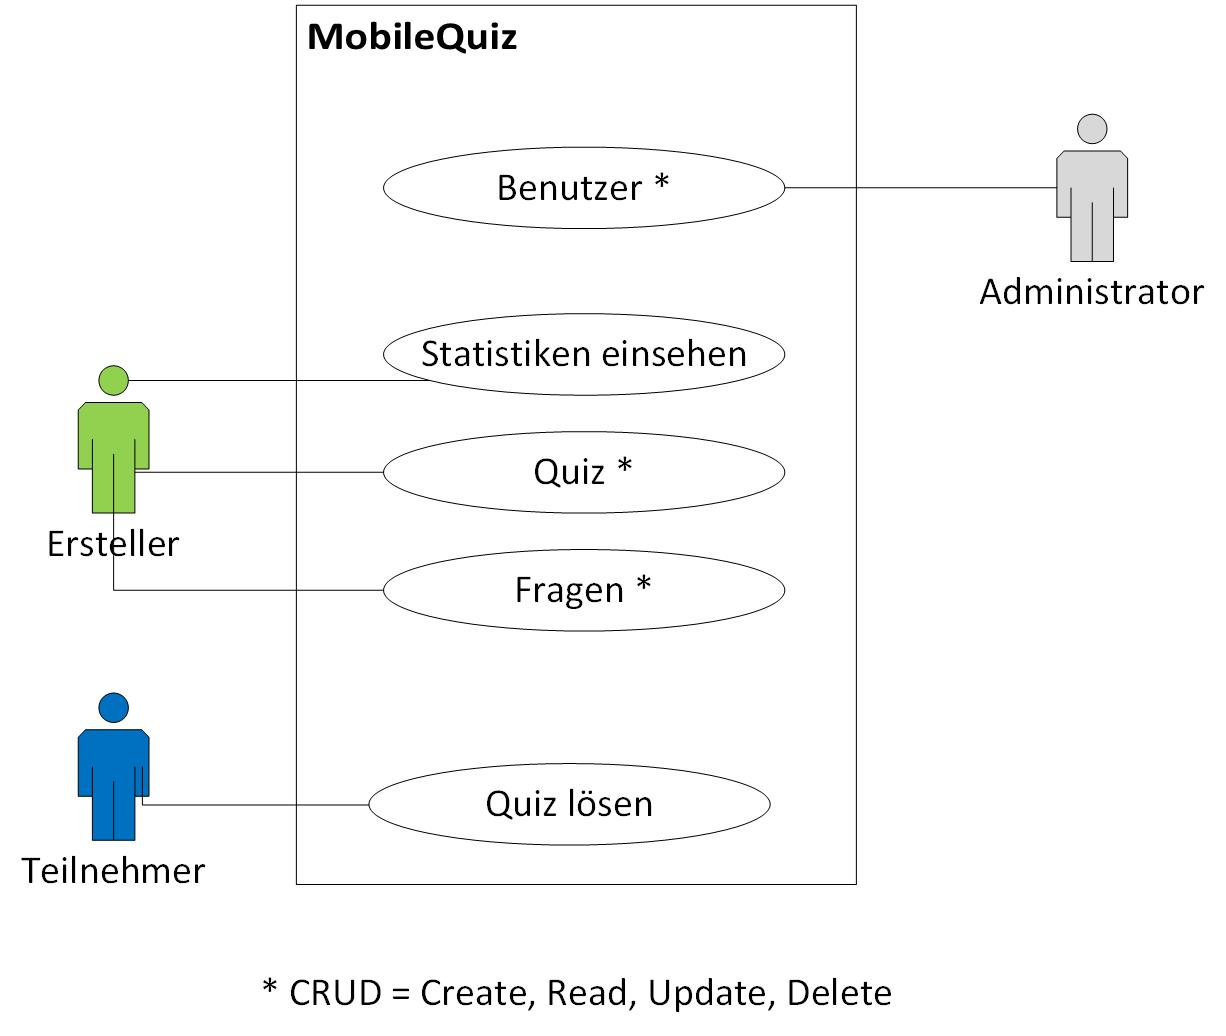
\includegraphics[width=0.75\textwidth]
	{Images/MobileQuiz_Uebersicht.PNG}
	\caption{Übersicht der wichtigsten Funktionen des Mobile Quiz}
\end{figure}

%Stand Mobile Quiz \\
Stand vor der Studienarbeit umfasst Mobile Quiz inzwischen einige Funktionen, um Quizzes zu erstellen. Verbesserungspotentiale liegen allerdings noch in den Bereichen der Bedienbarkeit, im Bereich von neuen Fragetypen sowie in der Auswertung von Quizzes. Durch letzteres wäre es dem Dozenten ersichtlich, welche Teile des Stoffs gut verstanden wurden und bei welchen noch Nachholbedarf herrscht. Somit könnte die Vorlesungszeit effizienter genutzt werden.

Die folgenden Bilder sollen die wichtigsten Ansichten in der alten Version des Mobile Quiz anzeigen. Die alte Version des Mobile Quiz ist unter \url{https://tlng.cnlab.ch/mobilequiz_v3} auffindbar.
\begin{figure}[H]
	\centering
	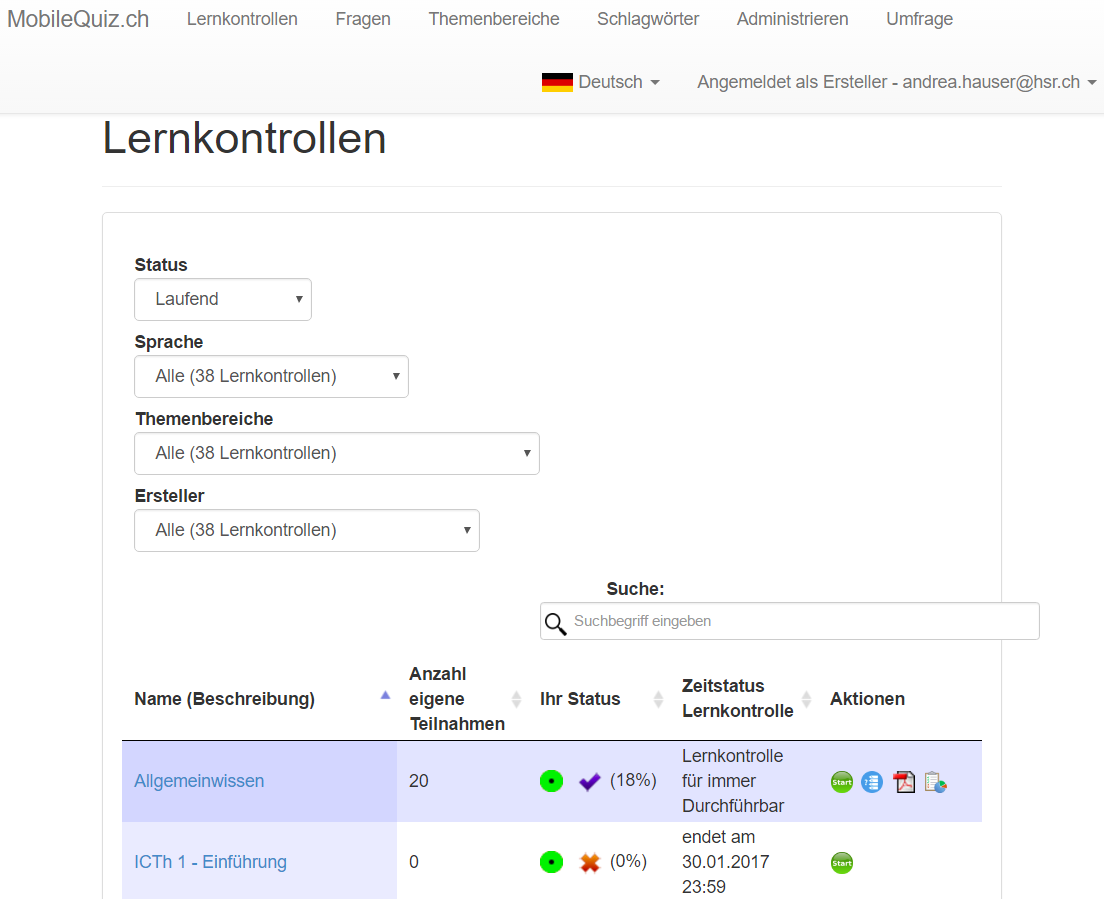
\includegraphics[width=0.75\textwidth]
	{Images/MobileQuizAlteVersionStartseiteErsteller.png}
	\caption{Ansicht der alten Mobile Quiz Startseite}
	\cite{mobilequiz.ch}
\end{figure}

\begin{figure}[H]
	\centering
	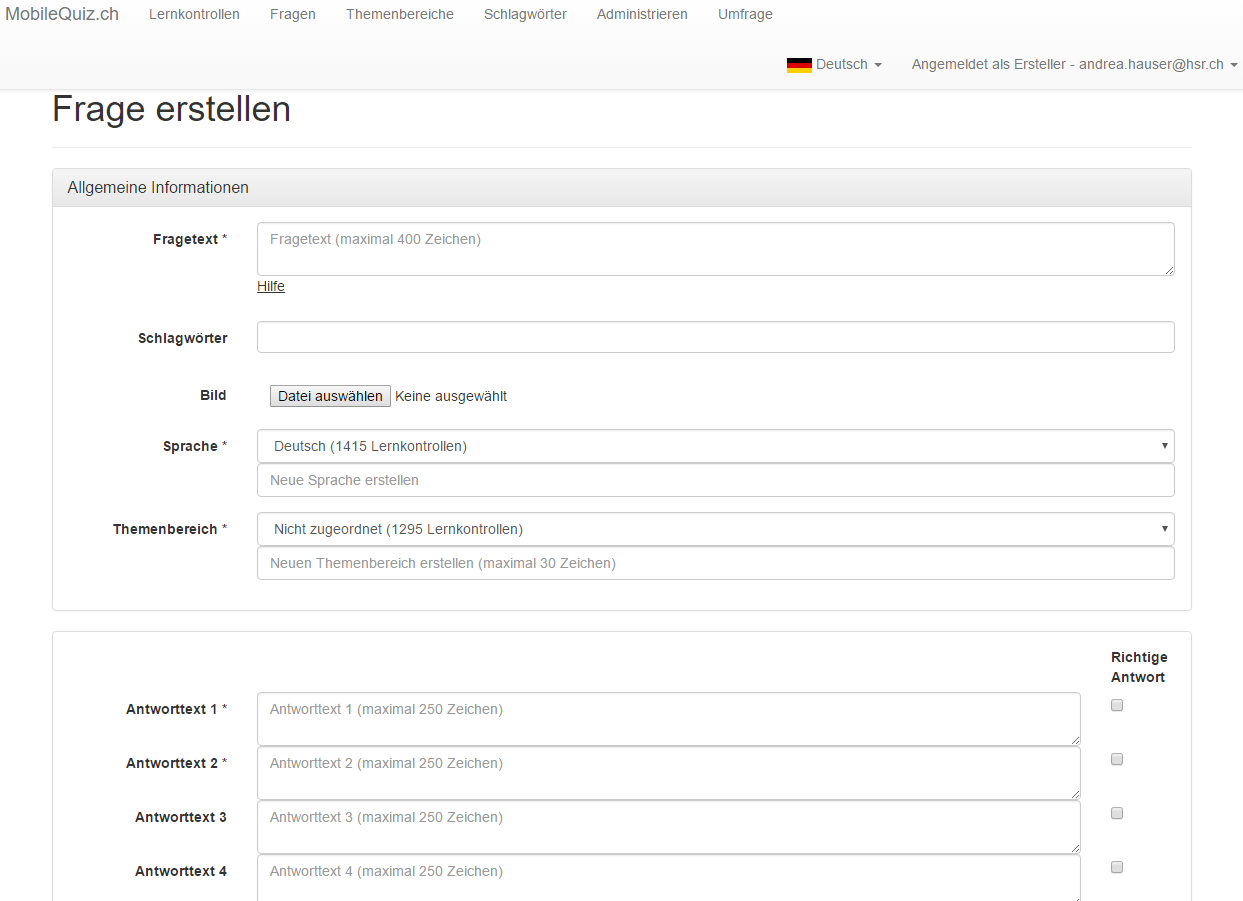
\includegraphics[width=0.75\textwidth]
	{Images/MobileQuizAlteVersionFrageErstellen.png}
	\caption{Ansicht der alten Mobile Quiz Fragen-Erstellungsseite}
	\cite{mobilequiz.ch}
\end{figure}

\begin{figure}[H]
	\centering
	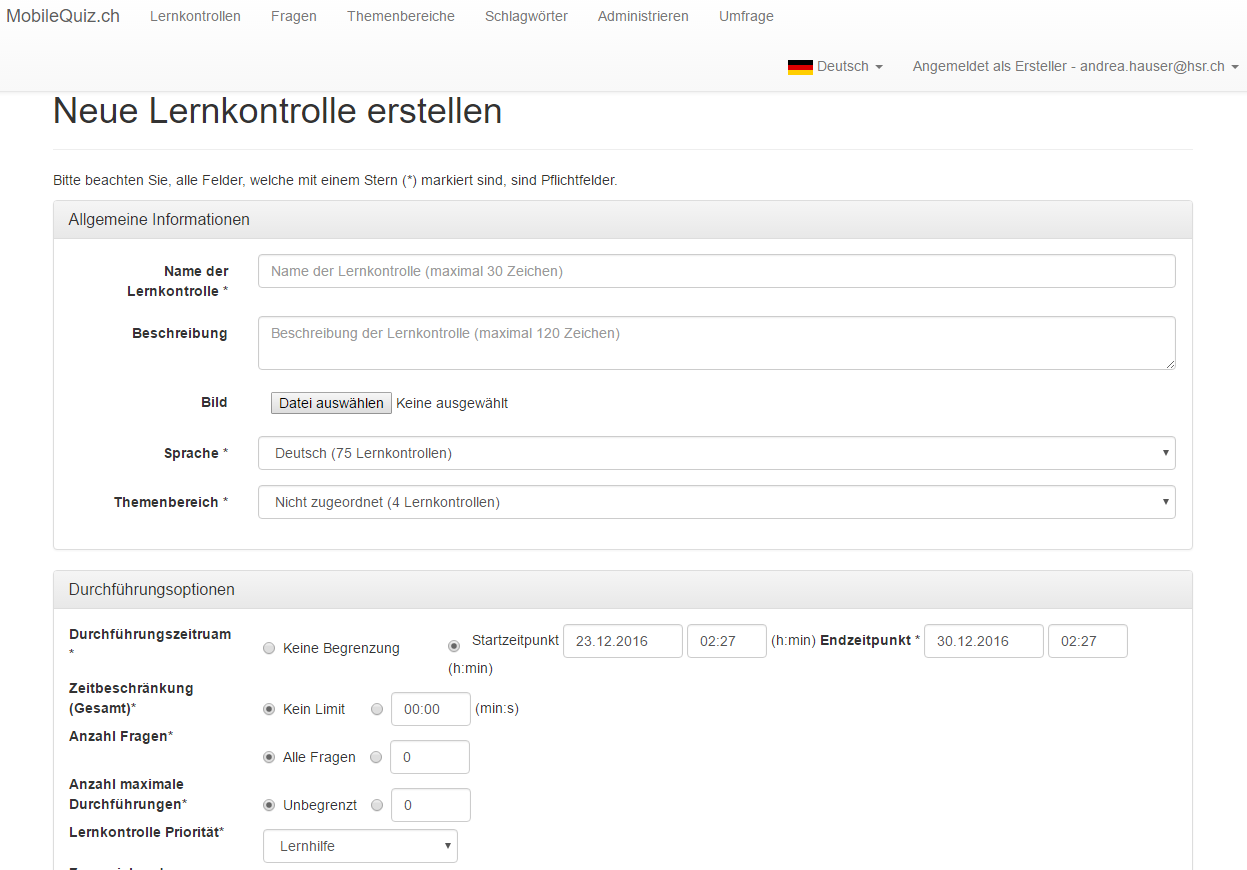
\includegraphics[width=0.75\textwidth]
	{Images/MobileQuizAlteVersionQuizErstellen.png}
	\caption{Ansicht der alten Mobile Quiz Quiz-Erstellungsseite}
	\cite{mobilequiz.ch}
\end{figure}

\begin{figure}[H]
	\centering
	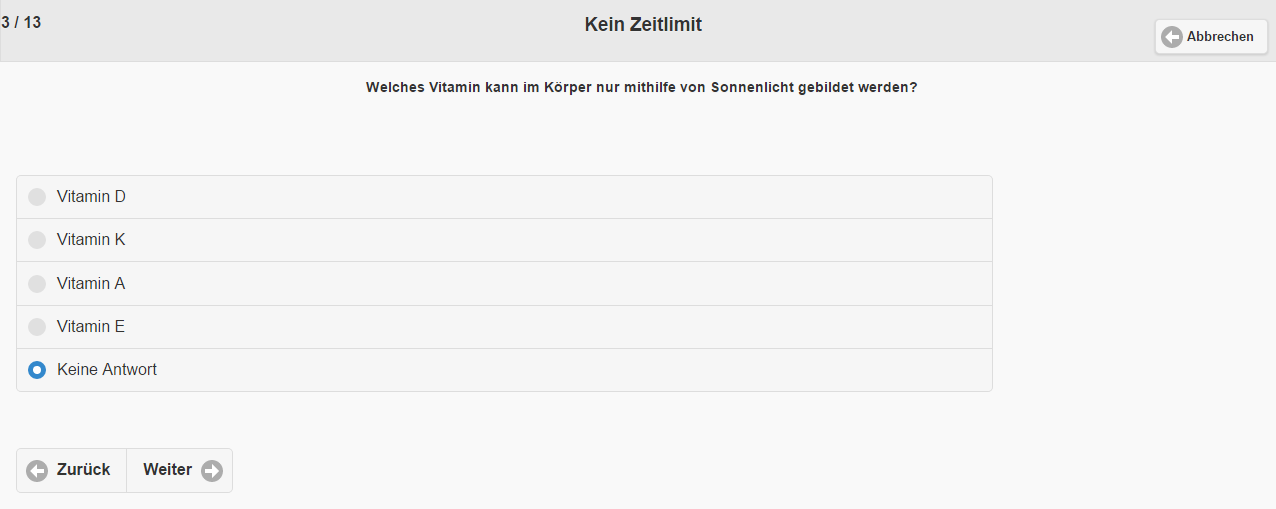
\includegraphics[width=0.75\textwidth]
	{Images/MobileQuizAlteVersionQuizDurchfuehrung.png}
	\caption{Ansicht der alten Mobile Quiz Quiz-Durchführungsseite}
	\cite{mobilequiz.ch}
\end{figure}

%In dieser Arbeit wird XY umgesetzt.
In dieser Arbeit die bessere Bedienbarkeit für Ersteller und Teilnehmer umgesetzt. Es wird dabei immer auch geschaut, dass die Mobile Version der Website bedienbar ist. Zudem werden neue Funktionalitäten, wie zum Beispiel das neue Excel für den Fragen-Import oder auch ein neuer Fragetyp implementiert.

\bigskip

%Übersicht Kapitel \\
Im folgenden Kapitel wird das bestehende Produkt genauer beschrieben und es wird darauf eingegangen, wie die Inbetriebnahme voranging. Das Kapitel drei befasst sich mit den zu Beginn vorgenommen Analysen im Bereich ähnliche Arbeiten, den eigenen Tests mit Mobile Quiz und der Umfeldanalyse. Im darauf folgenden Kapitel sind die erarbeiteten Konzepte zum Gruppenmanagement, den neuen Fragetypen und den Statistiken und Auswertungen zu finden. Das Kapitel Design zeigt die wichtigsten Überlegungen zu den Seitenneugestaltungen auf. Im darauf folgenden Kapitel Software Engineering werden die vorgenommen Datenbankänderungen beschrieben. Das Kapitel sieben befasst sich dann mit der Beschreibung der Implementation. Im Kapitel acht werden die Folgearbeiten beschrieben. Das nächste Kapitel setzt sich mit dem Qualitätsmanagement auseinander. Abgeschlossen wird der Hauptteil mit dem Kapitel zehn Schlussfolgerung.